Solve the heat equation $u_{xx} = u_t$ on the domain $\Omega = [0, 1]$ with initial temperature distribution 
$u(x, 0) = x$ and Neumann boundary conditions $u_x(0, t) = u_x(1, t) = 0$.

\begin{solution}\ \\\\
    We assume the full solution $u(x, t)$ to our system is the sum of a steady state function $u_s(x)$ and a transient 
    solution $v(x, t)$. Let $L = 1$. We begin with the observation that the fact that our Neumann boundary conditions 
    imply that no heat escapes or enters the system, and hence our steady-state temperature is simply the integral 
    average of the initial temperature distribution $u(x, 0) = x$:

    \begin{equation}
        u_s(x) = \int_0^1{u(x, 0)\; dx} = \int_0^1{x\; dx} = \frac{x^2}{2} \biggm\rvert_{0}^{1} = \frac{1}{2}.
    \end{equation}

    We thus need only solve for the transient solution $v(x, t)$.  To do so, we utilize separation of variables and 
    assume that $v(x, t)$ is the product of some function of $x$ and some function of $t$, i.e., 
    $v(x, t) = \phi(x) G(t)$. Substituting the product form of $v(x, t)$ into the heat equation yields:

    $$
    \frac{\partial^2}{\partial x^2} (\phi(x) G(t)) = \frac{\partial}{\partial t} (\phi(x) G(t)) \\
    $$

    and hence (observing that the partial derivatives on either side reduce to standard derivatives):

    $$
    G \frac{d^2 \phi}{d x^2} = \phi \frac{d G}{d t}.
    $$

    We divide both sides by $\phi G$ to find:

    $$
    \frac{1}{\phi} \frac{d^2 \phi}{d x^2} = \frac{1}{G} \frac{d G}{d t}.
    $$

    Since the left-hand side depends on $x$ only and the right-hand side on $t$, the left and right sides must be equal
    to some constant, which we denote $-\lambda^2$.

    The time-dependent side therefore becomes the first-order ODE:

    $$
    \frac{d G}{d t} = -\lambda^2 G.
    $$

    with solutions for any particular $\lambda$ given by:\footnote{
        We add subscripts here to $d_{\lambda}$ and $G_{\lambda}$ in order to emphasize that the exact form of the 
        function depends on the particular value which $\lambda$ takes.
    }

    $$
    G_{\lambda}(t) = d_{\lambda}e^{-\lambda^2 t}.
    $$

    Similarly, the space-dependent side becomes the following second-order ODE:

    $$
    \frac{d^2 \phi}{d x^2} = -\lambda^2 \phi.
    $$

    with the following general solution (where coefficient values again depend on $\lambda$):

    $$
    \phi(x) = b_{\lambda} \sin{(\lambda x)} + c_{\lambda} \cos{(\lambda x)}.
    $$

    We substitute our boundary condition $0 = v_x(0, t) = \phi_x(0)$ to find:

    $$
    0 = \phi_x(0) = b_{\lambda} \lambda \cos{(0)} - c_{\lambda} \lambda \sin{(0)} = b_{\lambda} \lambda.
    $$

    If we assume non-zero eigenvalues (since we recover the trivial solution otherwise), we find that $b_{\lambda} = 0$.
    Similarly, our Neumann boundary condition at $x = L$ yields:

    $$
    0 = \phi_x(L) = -c_{\lambda} \lambda \sin{(\lambda L)}.
    $$

    We again assume a non-trivial solution (i.e., $c_{\lambda} \neq 0$), and so we have that $\lambda$ must be:

    $$
    \lambda_n = \frac{n \pi}{L}, n \in \mathbb{N}
    $$

    Hence for any particular $n$, we have that $v_n(x, t) = \phi_n(x)G_n(t)$ is a solution to our PDE. Because arbitrary
    linear combinations of solutions are themselves solutions to the PDE by the principle of superposition, we have that
    our transient solution $v(x, t)$ is given by:\footnote{
        We reindex by letting $a_n = c_n d_n$.
    }

    \begin{equation}
    v(x, t) = \sum\limits_{n=1}^{\infty}{c_n \cos{\left(\frac{n \pi x}{L}\right)}} d_n e^{-\left(\frac{n \pi}{L}\right)^2 t}
            = \sum\limits_{n=1}^{\infty}{a_n \cos{(n \pi x)}} e^{-(n \pi)^2 t}.
    \end{equation}

    To determine our Fourier cosine coefficients $a_n$, we substitute (1) and (2) into our initial condition 
    $u(x, 0) = x$:

    \begin{align*}
        x = u(x, 0) = u_s(x) + v(x, 0) = \frac{1}{2} + \sum\limits_{n=1}^{\infty}{a_n \cos{(n \pi x)}}.
    \end{align*}

    We subtract $\frac{1}{2}$ from each side, multiply by $\cos{(m \pi x)}$ for some fixed $m \in \mathbb{N}$, and 
    integrate over our domain $\Omega = [0, 1]$ to find:\footnote{
        We may switch the order of integration and summation by the Dominated Convergence Theorem.
    }

    \begin{align*}
        \int_{0}^{1}{\left(x - \frac{1}{2}\right) \cos{(m \pi x)}\; dx}
            &= \int_{0}^{1}{\sum\limits_{n=1}^{\infty}{a_n \cos{(n \pi x)} \cos{(m \pi x)} }\; dx} \\
            &= \sum\limits_{n=1}^{\infty}{a_n \int_{0}^{1}{\cos{(n \pi x)} \cos{(m \pi x)}\; dx }} \\
            &= \frac{1}{2} a_m.
    \end{align*}

    Our Fourier cosine coefficients (for $m \ge 1$) are therefore given by:

    \begin{alignat*}{2}
        a_m &= 2 \int_{0}^{1}{\left( x - \frac{1}{2} \right) \cos{(m \pi x)}\; dx} \\
            % &= 2 \int_{0}^{1}{x \cos{(m \pi x)}\; dx} - \int_{0}^{1}{\cos{(m \pi x)}\; dx} \\
            &= 2 \int_{0}^{1}{x \cos{(m \pi x)}\; dx} - \frac{1}{m \pi} \sin{(m \pi x)} \biggm\rvert_{0}^{1} \\
            &= 2 \int_{0}^{1}{x \cos{(m \pi x)}\; dx} \\
            &= -\frac{2}{(m \pi)^2} \left(1 - (-1)^{m}\right).
    \end{alignat*}

    Substituting this expression into (2) yields our full solution $u(x, t)$:
    
    $$
    u(x, t) = u_s(x) + v(x, t) 
            = \frac{1}{2} + \sum\limits_{n=1}^{\infty}{-\frac{2}{(n \pi)^2} \left(1 - (-1)^{m}\right) \cos{(n \pi x)} e^{-(n \pi)^2 t}}
    $$

    For completeness, we plot two Fourier Series approximations to $u(x, 0) = x$:

    \begin{figure*}[h]
        \centering
        \begin{subfigure}[b]{0.475\textwidth}
            \centering
            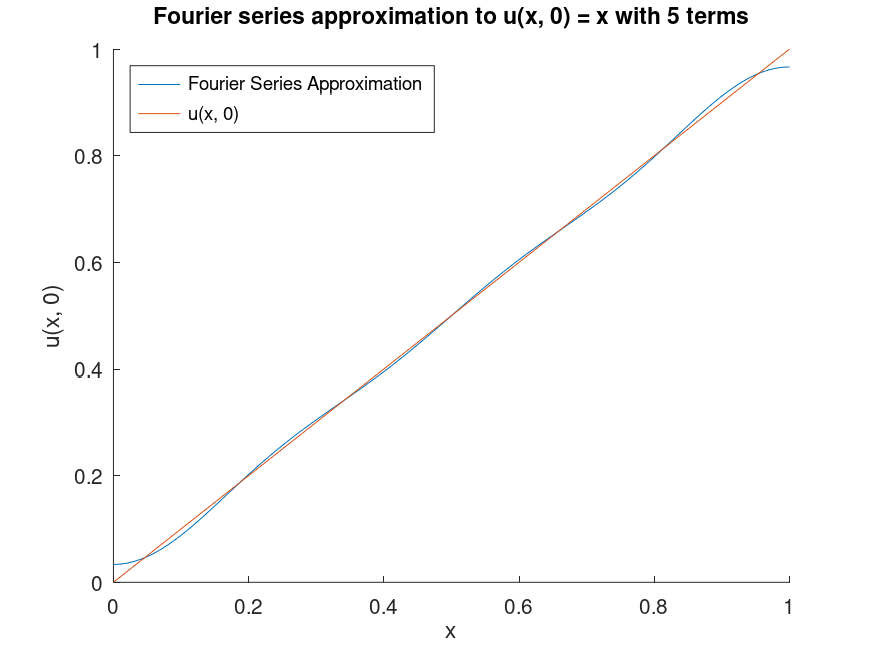
\includegraphics[width=\textwidth]{problem1_initial_fourier_series_solution_5_terms.png}
            \label{fig:problem1_5terms}
        \end{subfigure}
        \hfill
        \begin{subfigure}[b]{0.475\textwidth}
            \centering
            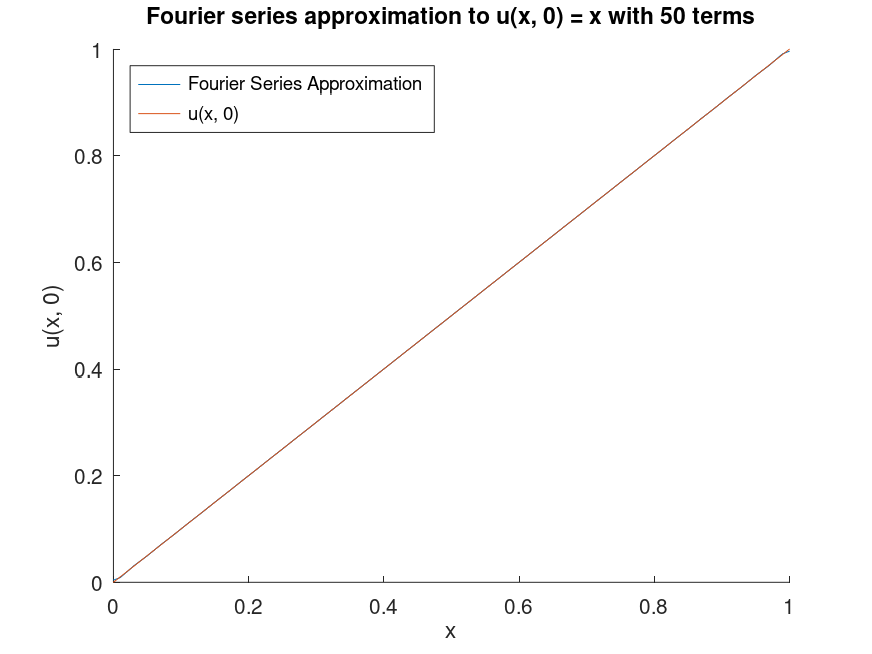
\includegraphics[width=\textwidth]{problem1_initial_fourier_series_solution_50_terms.png}
            \label{fig:problem1_50terms}
        \end{subfigure}
        \caption[Fourier Series solution]
        {\small Fourier Series approximation to $u_0(x) = x$} 
        \label{fig:fouriersoln}
    \end{figure*}

    \pagebreak

    Lastly, observe that as $t$ gets large, the dominant term in the series is at $n=1$ (i.e., 
    $-\frac{4}{\pi^2} \cos{(\pi x) e^{-\pi^2 t}}$) since the contribution from all even terms is zero and each 
    successive odd term is exponentially smaller than the last. In fact, even for $t = 0.2$ we see negligible 
    difference between 1 term and 255 terms:
    \ \\\\

    \begin{figure*}[h]
        \centering
        \begin{subfigure}[b]{0.475\textwidth}
            \centering
            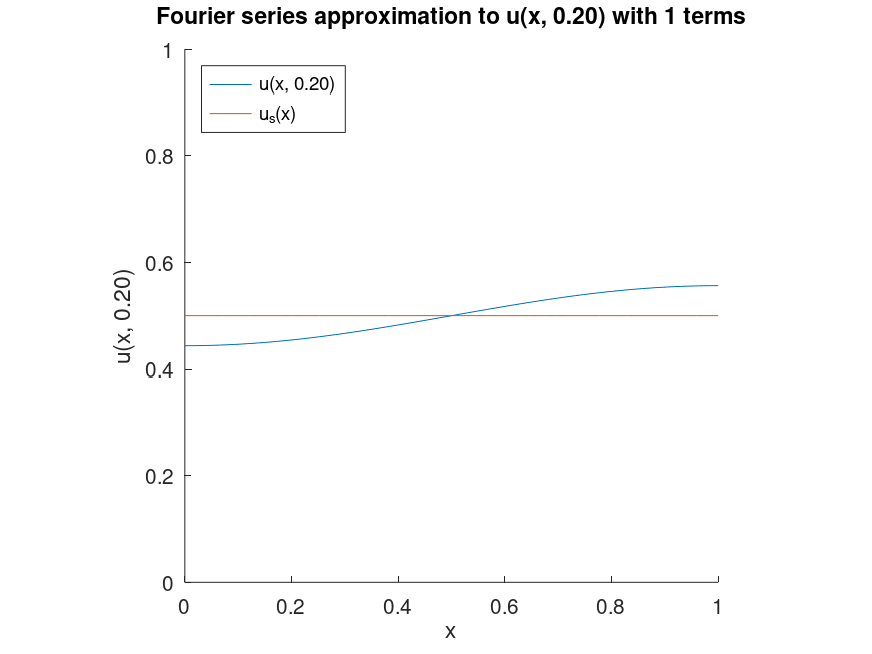
\includegraphics[width=\textwidth]{problem1_fourier_series_solution_1_terms_t_0.20.png}
            \label{fig:problem1_time_dependent_1term}
        \end{subfigure}
        \hfill
        \begin{subfigure}[b]{0.475\textwidth}
            \centering
            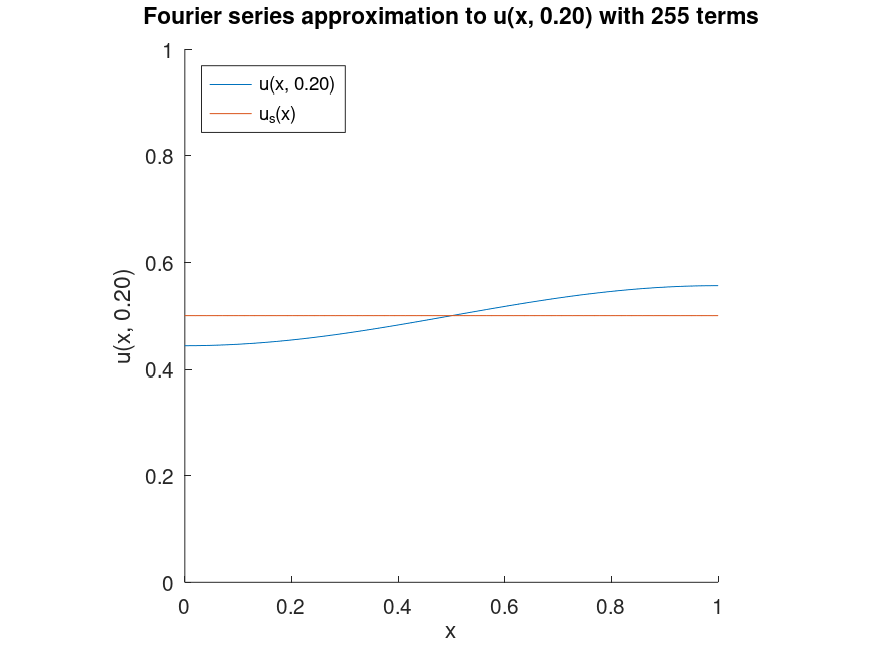
\includegraphics[width=\textwidth]{problem1_fourier_series_solution_255_terms_t_0.20.png}
            \label{fig:problem1_time_dependent_255terms}
        \end{subfigure}
        \caption[Fourier Series solution at $t = 0.2$]
        {\small Fourier Series approximation at $t = 0.2$} 
        \label{fig:fouriersoln}
    \end{figure*}
    \ \\
\end{solution}